
El proceso de cálculo que se va a seguir para la estimación completa de la instalación fotovoltaica conectada a red es el que se detalla en el libro de Óscar Perpiñán, tutor de este trabajo, denominado Energía Solar Fotovoltaica \cite{esf_book}. También se harán menciones a las presentaciones que se encuentran en el mismo enlace que el libro.\\

A lo largo de este capítulo, se utilizará el término \textbf{aplicación} para referirse a todo el conjunto de código relacionado tanto con proceso de obtención de todos los datos necesario como el de mostrar la información relevante al usuario.

\section{Obtención de datos del usuario}
Como se ha mencionado anteriormente, el objetivo principal de la aplicación es de realizar todos los cálculos que se necesitan para estimar una instalación fotovoltaica conectada a red, de la manera mas exacta posible,  en un emplazamiento concreto elegido por el usuario. Por tanto, el primer paso que tuve que dar con la aplicación fue la de obtener todos los datos necesarios para realizar dichos cálculos.
Estos datos son:
\begin{itemize}
\item Emplazamiento del usuario
\item Área, inclinación, orientación y nivel de suciedad de la superficie de instalación
\end{itemize}
\subsection{Emplazamiento del usuario}
Mas adelante, para poder obtener los datos de irradiación global en el plano horizontal, se necesitan los datos de latitud y longitud del sitio del que se quieren obtener dichos datos. Sin embargo, es poco intuitivo pedirle a un usuario que introduzca sus coordenadas, dado que la mayoría desconocen dichos datos.\\
Por lo tanto, la ruta que he tomado es la de pedirle al usuario su dirección, o una dirección cercana a su localización, y utilizar la API de Google Maps \footnote{\textit{API Google Maps}: Enlace interactivo al que se le pueden enviar los datos de una dirección y devuelve las coordenadas de latitud y longitud de un emplazamiento.  } para convertir dicha dirección en las coordenadas de latitud y longitud que necesito para poder extraer la irradiación que he mencionado antes.\\

Este proceso comienza por recoger los datos de la dirección, municipio y código postal a través del formulario que aparece en la página web.

Estos datos son recogidos en el código a través de un nombre único que han recibido:\\
\begin{lstlisting}[style=ES6, caption={Variables correspondientes a los tres campos}]
const addressInput = document.querySelector('#address');
const cityInput = document.querySelector('#city');
const postalInput = document.querySelector('#postal');
\end{lstlisting}

Una vez que tenemos estos datos recogidos en las variables, podemos pedir a la API de Google Maps las coordenadas de latitud y longitud de dicho emplazamiento encadenando las tres variables y una clave única de identificación,  para obtener un enlace único que se corresponde a dicha localización.\\

\begin{lstlisting}[style=ES6, label={lst:getCoordinates}, caption={Función encargada de solicitar los datos a la API}]
const getCoordinates = async () => {
	const address = addressInput.value.split(' ').join('+');
	const city = cityInput.value;
	const postal = postalInput.value;
	const requestURL = `${googleEndpoint}address=${address},${city},${postal}
										,spain&key=${googleApiKey}`;
	const response = await fetch(requestURL);
	const data = await response.json();
	const info = {
		formattedAdress: data.results[0].formatted_address,
		lat: data.results[0].geometry.location.lat,
		long: data.results[0].geometry.location.lng
	};

	return info;
};
\end{lstlisting}

La función de \textbf{getCoordinates} (\ref{lst:getCoordinates}) recoge el valor de la dirección y reemplaza los espacios con el signo + (formato requerido por la API) y lo concatena con el valor del campo de la ciudad y el código postal. Al final le añade una clave única que identifica la aplicación a la hora de establecer limites de uso y evitar abuso de la API.\\

Una vez creado este enlace único, el código lanza la petición al servicio y retorna con la información que es recogida y se guarda en dos variables \textbf{lat} y \textbf{long} para ser utilizadas posteriormente, a la hora de obtener los datos de irradiación global.

\subsection{Área, inclinación, orientación y nivel de suciedad de la superficie de instalación}

Además de las información de latitud y longitud del emplazamiento, el cálculo de la instalación también requiere de información relacionada con el área, la inclinación, la orientación y el nivel de suciedad de la superficie donde se va a realizar la instalación, para poder realizar una estimación lo mas exacta posible.

Estos valores son recogidos directamente de los campos de la pagina web, al igual que los campos anteriores, sin necesitar ningún trato especial:\\
\begin{lstlisting}[style=ES6, caption={Variables correspondientes a los campos indicados}]
const slope = document.querySelector('#slope');
const area = document.querySelector('#area');
const orientation = document.querySelector('#orientation');
const dirtLevel = document.querySelector('#dirt-level');
\end{lstlisting}

\section{Obtención de la irradiación global media en el plano horizontal}

El primer paso del cálculo de una instalación fotovoltaica es el de conocer la irradiación global media en el plano horizontal para el emplazamiento donde se va a realizar el cálculo. En la sección anterior se obtuvieron las coordenadas de latitud y longitud del emplazamiento introducido por el usuario.\\

En esta sección, se va a obtener la irradiación para las dichas coordenadas utilizando un servicio de ADRASE \footnote{\textit{ADRASE}: Acceso a Datos de irradiación Solar en España \url{http://www.adrase.com/}}, un proyecto realizado por el CIEMAT. Este servicio ofrece de manera gratuita y de uso libre, datos correspondientes a valores medios mensuales de irradiación global en el plano horizontal para toda la geografía española.\\

Los datos están disponibles a través de un mapa interactivo y de unos enlaces personalizados que incluyen la valores de latitud y longitud para los que se desea obtener dicha información. En esos enlaces se ofrecen los datos de irradiación global mínima, media y máxima en el plano horizontal.\\

Con el objetivo de no saturar la pagina de ADRASE y evitar error de funcionamiento de la aplicación debidos a la posibilidad de que la página desaparezca en un futuro, se ha realizado una descarga de los datos de la página, con un intervalo de 0.1 tanto en longitud como en latitud y se han guardado en una base de datos.De esta forma también se reducen los tiempos de cálculo en gran medida al tener un acceso casi instantáneo a los valores medios de irradiación. 
Una explicación detallada de como se ha realizado dicha descarga se incluye en el Anexo. ( ** TO DO Anexo con explicación **).
\newpage

\section{Naturaleza de la radiación solar}

\subsection{Radiación fuera de la atmósfera terrestre}
La radiación emitida por el Sol atraviesa el espacio vacío en todas las dirección sin sufrir pérdidas a causa de la interacción con los medios material. Sin embargo, la irradiancia solar, que se define como la densidad de flujo radiante solar, se ve atenuada por el cuadrado de la distancia. Parte de esta irradiancia es interceptada por la Tierra. Dada la relación entre la distancia con el Sol y el tamaño de nuestro planeta, se puede asumir que su valor es constante en toda la superficie exterior de la atmósfera. El valor promedio de esta irradiancia, según varias campañas de medición es de $B_{0} = 1367 \frac{W}{m^2}$.

Para calcular la irradiancia incidente en una superficie tangente a la atmosfera en una latitud, debemos tener en cuenta que la distancia entre la Tierra y el Sol varía a lo largo del año, debido a la excentricidad de la órbita elíptica que describe nuestro planeta. La ecuación para calcular dicho valor es:\\
\begin{equation}\label{eqn_B00}
B_0(0) = B_0\epsilon_0\cos\theta_{zs}
\end{equation}\\


Es importante resaltar que el valor de la irradiancia extra-atmosférica o extra-terrestre solo requiere consideraciones atmosféricas. Así, integrando la ecuación \ref{eqn_B00}, podemos calcular la irradiación diaria extra-terrestre con la ecuación obtenida:\\
\begin{equation}\label{eqn_B0d0}
B_{0d}(0)=-\frac{T}{\pi}B_0\epsilon_0·(\omega_s\sin\phi\sin\delta + \cos\phi\cos\delta\sin\omega_s)
\end{equation}\\

Es posible demostrar que el promedio mensual de esta irradiación diaria coincide numéricamente con el valor de irradiación diaria correspondiente a los denominados días promedios, días en los que la declinación correspondiente coincide con el promedio mensual. Por tanto, podemos calcular el valor medio mensual de la irradiación diaria extra-atmosférica con el valor de la declinación de uno de los doce días promedio.

Estos doce días promedios son:

\begin{table}[ht]
\centering
\begin{tabular}{|l|l|l|l|l|l|l|l|l|l|l|l|l|}
\hline
Mes   & Ene & Feb & Mar & Abr & May & Jun & Jul & Ago & Sep & Oct & Nov & Dic \\ \hline
$d_n$ & 17  & 45  & 74  & 105  & 135  & 161  & 199  & 230  & 261  & 292  & 322 & 347  \\ \hline
\end{tabular}
\label{tab:dias_promedio}
\caption{Dias promedio}
\end{table}

Para calcular esta irradiación diaria, debemos calcular primero los diferentes componentes que forman parte de esta:
\begin{itemize}
\item $B_{0} = 1367 \frac{W}{m^2}$
\item Factor de corrección por excentricidad: $\epsilon_0 = 1 + 0,033 · \cos(\frac{2\pid_n}{365})$

En código se representa de la siguiente manera:
\begin{lstlisting}[style=ES6, caption={Factor de corrección por excentricidad}]
		const exct = 1 + 0.033 * Math.cos((2 * Math.PI * elem.normalDay) / 365)
\end{lstlisting}
\item Ecuación de Cooper para la declinación: $\delta = 23,45\deg · \sin(\frac{2\pi·(d_n+284)}{365})$

En código se representa de la siguiente manera:
\begin{lstlisting}[style=ES6, caption={Ecuación de Cooper para declinación}]
		const decl = 23.45 * Math.sin((2 * Math.PI * (elem.normalDay + 284)) / 365)
\end{lstlisting}
\item Cenit Solar: $\cos(\theta_{zs}) = \cos(\delta)\cos(\omega)\cos(\phi) + \sin(\delta)sin(\phi)$\\

Para el calculo del cenit solar, hay que tener en cuenta que varía en función de la hora del día, así que se deberá calcular un valor para cada una de las 24h del día, con la diferencia de que en el cálculo, las horas irán de -12 a 12 en lugar de 0 a 23 y además, tendremos que convertir las horas a ángulos multiplicando por 15$\deg$. De tal manera, que en código, el calculo del cenit solar, tendrá ésta representación:\\
\begin{lstlisting}[style=ES6, caption={Cálculo del cenit solar}]
		for (let h = -12; h < 12; h++) {
			const cosZenit =
				Math.cos(deg2rad(elem.decl)) * Math.cos(deg2rad(h * 15)) * 	
					  Math.cos(deg2rad(newData.latitude)) +
				Math.sin(deg2rad(elem.decl)) * Math.sin(deg2rad(newData.latitude))
			const zenitVal = rad2deg(Math.acos(cosZenit))
		}
\end{lstlisting}
\end{itemize}

Aplicando estos cálculos a la ecuación \ref{eqn_B0d0} podemos calcular el valor de la irradiancia extra-terrestre diaria $B_{0d}(0)$ con la siguiente expresión:
\begin{lstlisting}[style=ES6, caption={Equación para B0d0}]
		const B0d0 =
			-(24 / Math.PI) *
			B0 *
			elem.exct *
			(elem.ws * Math.sin(deg2rad(newData.latitude)) * Math.sin(deg2rad(elem.decl)) +
				Math.cos(deg2rad(elem.decl)) * Math.cos(deg2rad(newData.latitude)) * 
				Math.sin(elem.ws))
\end{lstlisting}
donde:
\begin{itemize}
\item B0: valor contante de 1367 $W/m^2$
\item exct: excentricidad
\item ws: ángulo amanecer
\item decl: declinación
\end{itemize}
Para el cálculo de la irradiancia solar que finalmente incide en una superficie localizada en la corteza terrestre será útil distinguir tres componentes diferenciados, comúnmente denominados:

\begin{itemize}
\item Radiación Directa, \textit{B}: representa la fracción procedente en linea directa del Sol.
\item Radiación Difusa, \textit{D}: representa toda la radiación procedente de todo el cielo, excepto del sol, y por tanto incluye todos los rayos dispersados por la atmósfera. Es una radiación que depende del estado de la atmósfera, y variará en función de las condiciones climatológicas.
\item Radiación del albedo, \textit{R}: es aquella fracción de la radiación procedente de la reflexión con el suelo. Habitualmente, supone una contribución muy pequeña, que en algunos casos, como el de este proyecto, puede ser despreciada.
\end{itemize}

La suma de las tres componentes constituyen la denominada irradiancia global:
\begin{equation}
G=B+D+R
\end{equation}
\label{equation:eqn_global_radiation}
\subsubsection{Nomeclatura}

Es importante distinguir, dentro de las ecuaciones que modelan el comportamiento de la radiación solar, la forma de indicar cada componente de la irradiancia, el instante o el período en el que se recibe. 

Es recomendable leer estas expresiones en el orden período, forma, tiempo y lugar utilizando el formato de nomenclatura de la siguiente ecuación
\begin{equation}
	Forma_{tiempo, promedio}(lugar)
\end{equation}

Para expresar el lugar de incidencia caben las siguiente posibilidades:
\begin{itemize}
\item (Orientación, Inclinación) : ($\beta , \alpha$)
\item (Horizontal) : (0)
\item (Superficie perpendicular al vector solar): ($n$)
\item (En el plano del generador): ($I$)
\end{itemize}

Por ejemplo, al escribir $B_{h}(0)$ leeremos irradiación directa (forma) horaria (tiempo) en el plano horizontal (lugar), mientras que $G_{d,m}(I)$ se lee media mensual (período) de la irradiación global (forma) diaria (tiempo) en el plano generador (lugar).\\

\section{Cálculo de componentes de radiación solar}

Para poder calcular la energía producida por un generador fotovoltaico, es necesario conocer la radiación solar que incide sobre la superficie de dicho generador. Para poder predecir la energía producida por éste en un tiempo futuro, el problema que se ha de resolver es estimar la irradiancia \footnote{\textbf{Irradiancia}: densidad de potencia de radiación solar incidente en una superficie. Unidades: $\frac{W}{m^2}$} que recibirá, a partir del comportamiento de la radiación solar en ese lugar.

En 1960, Liu y Jordan \cite{lj60} expusieron una forma de caracterizar la radiación solar en un lugar, mediante el indice de claridad $K_T$. Éste índice es la relación entre la radiación global y la extra-terrestre, ambas en el plano horizontal. La expresión de el indice de claridad diario es:\\

\begin{equation}
K_{Td} = \frac{G_d(0)}{B_{0d}(0)}
\end{equation}
mientras que el indice de claridad mensual es la relación entre las medias mensuales de irradiación diaria:
\begin{equation}
K_{Tm} = \frac{G_{d,m}(0)}{B_{0d,m}(0)}
\end{equation}

Partiendo de los datos obtenidos en la sección anterior debemos calcular las componentes de irradiación directa y difusa en el plano horizontal y después realizar el paso al plano inclinado.

Un esquema resumido del proceso se indica a continuación:

\begin{figure}[ht]
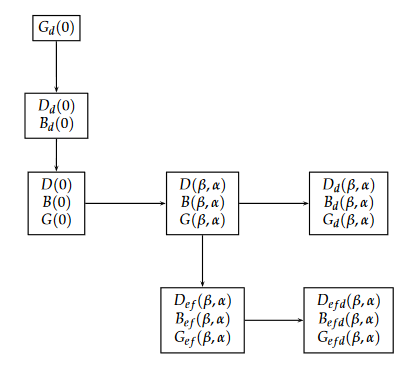
\includegraphics[scale=0.7]{32_ESFBOOK_1}
\centering
\caption{Procedimiendo de cálculo (Figura 3.3 pág 31 \cite{esf_book})}
\label{fig:fig_1}
\end{figure}

En la figura \ref{fig:fig_1} se muestra el proceso de cálculo que se va a seguir para llegar a los valores necesarios para poder estimar la potencia y energía de la instalación.

Los pasos descritos son:
\begin{enumerate}
	\item Separar la irradiación global diaria en el plano horizontal en sus componentes de irradiación difusa y directa.
	\item Convertir la irradiación diaria a un perfil horario de irradiación global, directa y difusa en en plano horizontal.
	\item Pasar del perfil horario en el plano horizontal a un perfil con la inclinación y orientación indicada por el usuario.
	\item Aplicar las pérdidas relacionadas con el ángulo de incidencia y el nivel de suciedad.
	\item Volver a convertir el perfil horario a unos valores diarios de irradiación global, difusa y directa.
\end{enumerate}

\subsection{Separación de la irradiación global diaria en sus componentes}

Como se ha indicado anteriormente, el primer paso del proceso de cálculo es el de separar la irradiación global diaria en en plano horizontal en sus dos componentes, la directa y la difusa.

















